\documentclass{article}
\usepackage[utf8]{inputenc}
\usepackage{amsmath}
\usepackage{amsfonts}
\usepackage{amssymb}
\usepackage{tikz}
\usetikzlibrary{arrows.meta, positioning, shapes.geometric, automata}

\begin{document}

\begin{flushleft}
FNL 2026, Renaud Richardet \hfill

\begin{tikzpicture}[baseline=(logo.base)]
    \node (logo) at (0,0) {};
    \fill[cyan!40] (0.1,0.2) circle (0.15);
    \fill[magenta!40] (0.3,0.2) circle (0.15);
    \fill[yellow!60] (0.2,0.4) circle (0.15);
    \node[anchor=west, font=\tiny\sffamily, align=left] at (0.5,0.25) {Informatique et systèmes\\de communication ISC \tiny\textsf{R}};
\end{tikzpicture}
\end{flushleft}

\vspace{1em}
{\large Nom: \underline{\text{REDACTED - REDACTED}}}

\vspace{2em}
{\huge Quizz automates finis}

\vspace{2em}
1. Quels mots sont acceptés par l'automate ci-dessous ?

\begin{center}
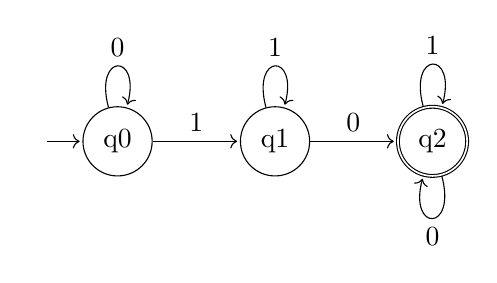
\begin{tikzpicture}[shorten >=1pt, node distance=2cm, on grid, auto]
    \node[state, initial, initial text=] (q0) {q0};
    \node[state] (q1) [right=of q0] {q1};
    \node[state, accepting] (q2) [right=of q1] {q2};

    \path[->]
    (q0) edge [loop above] node {0} ()
         edge node {1} (q1)
    (q1) edge [loop above] node {1} ()
         edge node {0} (q2)
    (q2) edge [loop above] node {1} ()
         edge [loop below] node {0} ();
\end{tikzpicture}
\end{center}

[ ] 011 \\
[$\checkmark$] 1010 \\
[ ] 111 \\
[ ] 0001

\vspace{2em}
2. L'automate ci-dessous accepte un nombre impair de ``a''

\begin{center}
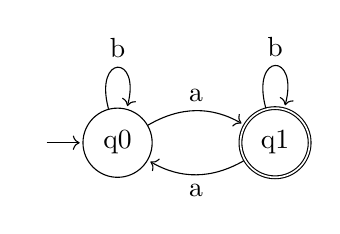
\begin{tikzpicture}[shorten >=1pt, node distance=2cm, on grid, auto]
    \node[state, initial, initial text=] (q0) {q0};
    \node[state, accepting] (q1) [right=of q0] {q1};

    \path[->]
    (q0) edge [loop above] node {b} ()
         edge [bend left] node {a} (q1)
    (q1) edge [loop above] node {b} ()
         edge [bend left] node {a} (q0);
\end{tikzpicture}
\end{center}

[$\checkmark$] vrai \\
[ ] faux

\vspace{2em}
3. Quels mots sont acceptés par l'automate ci-dessous ?

\vspace{1em}
[ ] aaaba \\
[ ] aaaa \\
[$\checkmark$] aaab \\
[ ] baab

\newpage

\begin{flushleft}
FNL 2026, Renaud Richardet \hfill

\begin{tikzpicture}[baseline=(logo.base)]
    \node (logo) at (0,0) {};
    \fill[cyan!40] (0.1,0.2) circle (0.15);
    \fill[magenta!40] (0.3,0.2) circle (0.15);
    \fill[yellow!60] (0.2,0.4) circle (0.15);
    \node[anchor=west, font=\tiny\sffamily, align=left] at (0.5,0.25) {Informatique et systèmes\\de communication ISC \tiny\textsf{R}};
\end{tikzpicture}
\end{flushleft}

\vspace{1em}
4. Dessinez un AFD qui accepte tous les mots avec \\
au moins 1 « a » et exactement 2 « b » \\
N'utilisez pas de ``shortcuts'' (!, @, e) dans les transitions, mais seulement a et/ou b.

\vspace{2em}
\begin{center}
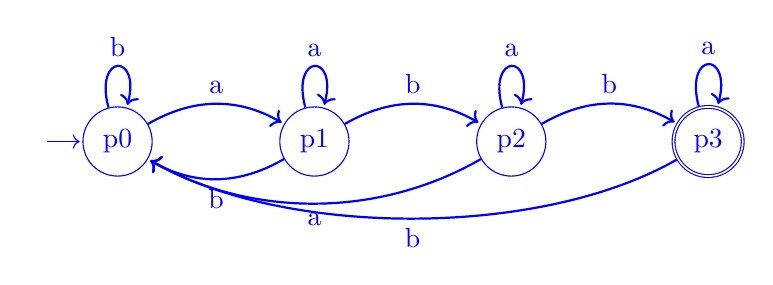
\begin{tikzpicture}[shorten >=1pt, node distance=2.5cm, on grid, auto, blue]
    \node[state, initial, initial text=] (p0) {p0};
    \node[state] (p1) [right=of p0] {p1};
    \node[state] (p2) [right=of p1] {p2};
    \node[state, accepting] (p3) [right=of p2] {p3};

    \path[->, thick]
    (p0) edge [loop above] node {b} ()
         edge [bend left] node {a} (p1)
    (p1) edge [loop above] node {a} ()
         edge [bend left] node {b} (p2)
         edge [bend left] node {b} (p0) % Transcription of a messy back arrow
    (p2) edge [loop above] node {a} ()
         edge [bend left] node {b} (p3)
         edge [bend left, distance=1.5cm] node {a} (p0) % Transcription of another messy arrow
    (p3) edge [loop above] node {a} ()
         edge [bend left, distance=2cm] node {b} (p0); % Transcription of a large return arrow
\end{tikzpicture}
\end{center}

\vspace{2em}
5. Pour chaque pattern du jeu de la vie ci-dessous, dessinez les prochaines phases \\
et indiquez si le pattern est stable ou cyclique (dans ce cas, indiquez la taille du \\
cycle).

\newcommand{\gamegrid}[2]{
    \begin{tikzpicture}[scale=0.25]
        \draw[step=1, gray, thin] (0,0) grid (10,10);
        #1 % Pre-filled yellow
        #2 % Student blue marks
    \end{tikzpicture}
}

\begin{minipage}{0.24\textwidth}
\centering
\text{cyclique} \\
\gamegrid{
    \fill[yellow] (4,5) rectangle (5,6);
    \fill[yellow] (5,4) rectangle (6,5);
    \fill[yellow] (5,6) rectangle (6,7);
    \fill[yellow] (6,5) rectangle (7,6);
}{} \\
\gamegrid{}{\fill[blue!40] (4,4) rectangle (5,5); \fill[blue!40] (4,5) rectangle (5,6); \fill[blue!40] (4,6) rectangle (5,7); \fill[blue!40] (5,4) rectangle (6,5); \fill[blue!40] (5,6) rectangle (6,7); \fill[blue!40] (6,4) rectangle (7,5); \fill[blue!40] (6,5) rectangle (7,6); \fill[blue!40] (6,6) rectangle (7,7);} \\
\gamegrid{}{\fill[blue!40] (4,5) rectangle (5,6); \fill[blue!40] (5,4) rectangle (6,5); \fill[blue!40] (5,6) rectangle (6,7); \fill[blue!40] (6,5) rectangle (7,6);}
\end{minipage}
\begin{minipage}{0.24\textwidth}
\centering
\text{stable} \\
\gamegrid{
    \fill[yellow] (2,3) rectangle (4,4);
    \fill[yellow] (2,4) rectangle (3,5);
    \fill[yellow] (5,5) rectangle (7,6);
    \fill[yellow] (6,6) rectangle (7,8);
}{} \\
\gamegrid{}{\fill[blue!40] (2,3) rectangle (4,4); \fill[blue!40] (2,4) rectangle (3,5); \fill[blue!40] (4,4) rectangle (5,5); \fill[blue!40] (5,5) rectangle (7,6); \fill[blue!40] (6,6) rectangle (7,8);} \\
\gamegrid{}{}
\end{minipage}
\begin{minipage}{0.24\textwidth}
\centering
\text{cyclique} \\
\gamegrid{
    \fill[yellow] (3,4) rectangle (6,5);
    \fill[yellow] (3,5) rectangle (4,7);
    \fill[yellow] (6,6) rectangle (9,7);
    \fill[yellow] (8,4) rectangle (9,6);
}{} \\
\gamegrid{}{} \\
\gamegrid{}{}
\end{minipage}
\begin{minipage}{0.24\textwidth}
\centering
\text{stable} \\
\gamegrid{
    \fill[yellow] (3,4) rectangle (5,6);
    \fill[yellow] (6,6) rectangle (8,8);
}{} \\
\gamegrid{}{} \\
\gamegrid{}{}
\end{minipage}

\end{document}
